\documentclass[a4paper,12pt]{article}
\usepackage[utf8]{inputenc}
\usepackage[T1]{fontenc}
\usepackage[ngerman]{babel}
\usepackage{lipsum}
\usepackage{titlesec} 
\usepackage[a4paper,left=2.5cm,right=2.5cm,top=2.5cm,bottom=2.5cm]{geometry}
\usepackage{setspace} 
\usepackage{parskip} 
\usepackage{graphicx} 


\title{Verteilte Systeme - Blackout}
\author{Axel Walz, Tarek Bürner, David Langner}
\date{\today}


\titleformat{\section}[block]{\normalfont\Large\bfseries}{\thesection}{1em}{}
\titlespacing*{\section}{0pt}{\baselineskip}{\baselineskip}
\let\stdsection\section
\renewcommand\section{\newpage\stdsection}

\begin{document}

%\pagestyle{empty}
\onehalfspacing 

\maketitle

\newpage 
\tableofcontents
\newpage 
\pagestyle{plain}
\pagenumbering{arabic}

\section{Einführung Blackout}
Das Buch "Blackout" von Marc Elsberg beschreibt ein fiktives Szenario, in dem ein großflächiger Stromausfall Europa und Nordamerika lahmlegt. Die Geschichte beginnt mit dem plötzlichen Zusammenbruch des Stromnetzes, der durch einen koordinierten Cyberangriff auf die kritische Infrastruktur verursacht wird. Dieser Angriff zeigt die Verwundbarkeit moderner, stark vernetzter und verteilter Systeme.

Im Kontext verteilter Systeme beleuchtet das Buch mehrere wichtige Aspekte. Es zeigt, wie anfällig verteilte Systeme für Cyberangriffe sind, indem die Angreifer Schwachstellen in der Software und den Kommunikationsprotokollen der Stromnetze ausnutzen, um eine Kettenreaktion auszulösen, die zu einem großflächigen Blackout führt. Dies unterstreicht die Notwendigkeit robuster Sicherheitsmaßnahmen und regelmäßiger Sicherheitsüberprüfungen in verteilten Systemen.

Ein zentrales Thema des Buches ist die Bedeutung von Redundanz und Fehlertoleranz in verteilten Systemen. Der Ausfall eines Teils des Stromnetzes sollte nicht zum Zusammenbruch des gesamten Systems führen. Das Buch zeigt jedoch, dass viele Systeme nicht ausreichend redundant ausgelegt sind, was zu katastrophalen Folgen führen kann.

Die Koordination und Kommunikation zwischen verschiedenen Teilen des Stromnetzes sind entscheidend für die Stabilität und Wiederherstellung des Systems. Das Buch beschreibt, wie Kommunikationsausfälle und mangelnde Koordination die Situation verschlimmern und die Wiederherstellung verzögern. Dies betont die Notwendigkeit effektiver Kommunikationsprotokolle und -strategien in verteilten Systemen.

Schließlich behandelt das Buch die Herausforderungen der Wiederherstellung nach einem großflächigen Ausfall. Die Resilienz eines verteilten Systems hängt von seiner Fähigkeit ab, sich schnell und effizient von Störungen zu erholen. Das Buch zeigt, dass die Wiederherstellung komplex und zeitaufwändig sein kann, insbesondere wenn die Systeme nicht auf solche Szenarien vorbereitet sind.

Insgesamt bietet "Blackout" eine spannende und lehrreiche Perspektive auf die Herausforderungen und Risiken, die mit verteilten Systemen verbunden sind. Es unterstreicht die Notwendigkeit robuster Sicherheitsmaßnahmen, Redundanz, effektiver Kommunikation und Resilienz, um die Stabilität und Zuverlässigkeit kritischer Infrastrukturen zu gewährleisten.

\section{Event Driven Architecture}
\subsection{Grundlagen und Prinzipien}
Die Event Drive Architecture ist ein Architekturstil, der zu mehr Effizienz in Anwendungen führt. Dabei stehen Ereignisse im Vordergrund. Ereignisse beziehen sich immer auf die Veränderung eines Zustandes wie zum Beispiel die Veränderung einer gemessen Temperatur oder der Eingang eines HTTP Requests.
Als Ereignisgesteuert (event-driven) gilt ein System, wenn Aktionen innerhalb dieses Systems nicht einer festen Abfolge entsprechen sondern immer dynamisch eine Reaktion auf das Eintreffen ein solchen Ereignisses ausgeführt werden.
Der zentrale Ablauf von ereignisgesteuerten Systemen besteht aus drei Schritten: Erkennen, Verarbeiten und Reagieren. \cite[S. 48f]{Bruns2010}

\textit{Erkennen}: In diesem Schritt wird ein Ereignis identifiziert, das eine Zustandsänderung signalisiert, wie z.B. eine Temperaturänderung oder ein eingehender HTTP-Request. Entscheidend hierfür ist, dass Ereignisse ohne Zeitverzögerung und somit unmittelbar nach ihrem Auftreten erkannt werden.

\textit{Verarbeiten}: Das erkannte Ereignis wird während der Analyse abstrahiert, klassifiziert oder verworfen. Es wird darauf geachtet, dass bestimmte Beziehungen oder Abfolgen zwischen Ereignissen erkannt werden, die eine Aktion auslösen würde.

\textit{Reagieren}: Schließlich werden die vorbereiteten Aktionen ausgeführt, um auf das Ereignis zu reagieren und den neuen Zustand zu verarbeiten. Häufig vorkommende Reaktionen sind das Schicken von Warnmeldungen oder die Initiierung von Aktionen durch menschliche Benutzer. 

Um ein solches System zu realisieren muss während dem Erstellen der Softwarearchitektur darauf geachtet werden, dass es ohne eine zentrale Steuerung konzipiert wird.
Reagieren: Schl ießlich werden die vorbereiteten Aktionen ausgeführt, um auf das Ereignis zu reagieren und den neuen Zustand zu verarbeiten. \cite[S. 50]{Bruns2010}

Da nicht jedes System, das Ereignisse beinhaltet direkt die Kriterien für ein Event Driven System erfüllt, gibt es verschiedene zwei Eigenschaften, die ein ereignisgesteuerts System erfüllen muss. \newline
\textit{1. Verarbeitungsmodell:} \newline
Das Verarbeitungsmodell, das jedem ereignisgesteuerten Systemn zugrunde liegt, besteht aus drei ELementen: Ereignisquelle, Ereignissenke und Ereignisobjekt.
Ereignisquelle: Die Ereignisquelle, auch als Produzent bezeichnet, erkennt relevante Informationen und erzeugt Ereignisse, die als Nachrichten an einen Mediator gesendet werden. Der Mediator verteilt diese Nachrichten weiter, ohne dass die Ereignisquelle Details zur Verarbeitung oder zu den Empfängern kennen muss. Dadurch erreicht das System eine hohe Aktualität, da Ereignisse sofort nach ihrem Auftreten weitergeleitet werden.
Ereignissenke: Die Ereignissenke (Konsument) ist eine Komponente, die ein Ereignis empfängt und direkt darauf reagiert. Sobald ein Ereignis eintrifft, wird ein entsprechender Verarbeitungsvorgang ausgelöst.
Ereignisobjekt: Das Ereignisobjekt enthält nur Informationen über das Ereignis selbst, aber keine Details zur Reaktion darauf. Die Verarbeitung und die entsprechende Reaktion liegen vollständig bei der Ereignissenke. Dies verringert die Abhängigkeit zwischen Ereignisquelle und Ereignissenke was dazu führt, dass verschiedene Komponenten unabhängig voneinander auf dasselbe Ereignis reagieren können. \cite[S. 51f]{Bruns2010} \newline
Abbildung \ref{fig:Verarbeitungsmodell} veranschaulicht das Modell. 

\begin{figure}[h]
    \centering
    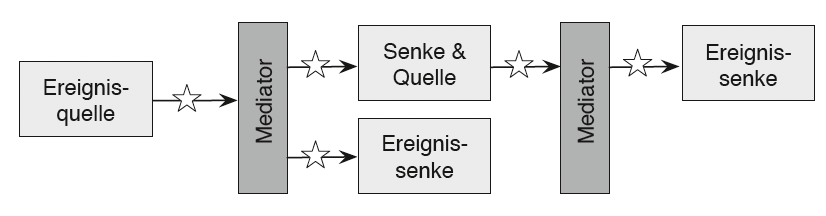
\includegraphics[width=0.8\textwidth]{images/Verarbeitungsmodell.png}
    \caption{Verarbeitungsmodell der Event Driven Architecture \cite[S. 52]{Bruns2010}}
    \label{fig:Verarbeitungsmodell}
\end{figure}

\textit{2. Kommunikationsmuster:} \newline
Das Kommunikationsmuster in einem ereignisgesteuerten System muss folgende Eigenschaften besitzen: Asynchronität, Publish/Subsribe-Interaktion und Push-Modus.
Asynchronität: Die Ereignisquelle sendet Nachrichten, ohne auf eine Antwort zu warten. Das bedeutet, dass Quelle und Empfänger unabhängig voneinander arbeiten können und nicht gleichzeitig aktiv sein müssen. Dadurch erhöht sich die Flexibilität und Effizienz der Kommunikation.
Publish/Subscribe-Interaktion: Die Ereignisquelle (“Publisher”) sendet Nachrichten an eine Middleware, und interessierte Empfänger (“Subscriber”) können diese Nachrichten abonnieren. Dies ermöglicht es mehreren Konsumenten, gleichzeitig auf dasselbe Ereignis zu reagieren.
Abbildung \ref{fig:PubSub} veranschaulicht das Modell.

\begin{figure}[h]
    \centering
    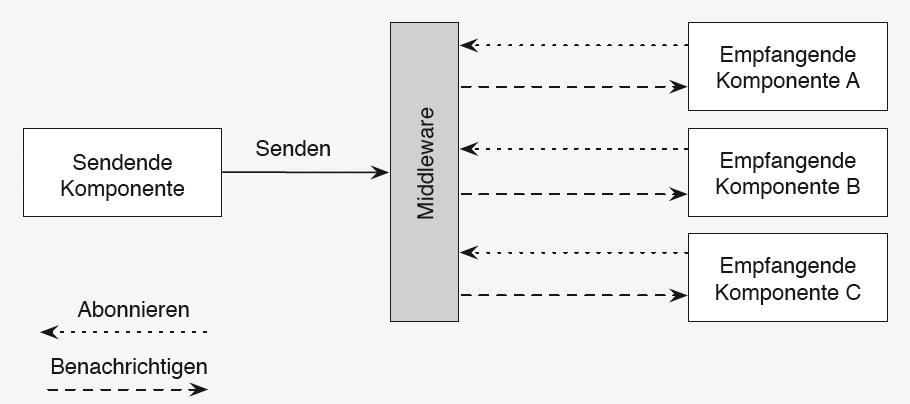
\includegraphics[width=0.8\textwidth]{images/Publish_Subscirbe.png}
    \caption{Publish/Subscirbe Interaktion \cite[S. 54]{Bruns2010}}
    \label{fig:PubSub}
\end{figure}
Push-Modus: Die Initiative zur Interaktion geht immer von der Ereignisquelle aus, die den Zeitpunkt des Nachrichtenaustauschs bestimmt. Dieses Push-basierte Modell ermöglicht eine hohe Entkopplung zwischen den Komponenten und fördert so die Skalierbarkeit und Interoperabilität des Systems. \cite [S. 53f]{Bruns2010}
\subsection{Beispielanwendungen in Bezug auf Blackout}
 \cite{example2023}

\section{Load Balancing}
\subsection{Grundlagen und Funktionsweise}
In Abbildung \ref{fig:LoadBalancing} ist ein Beispielhaftes Modell des Load Balancing in der Cloud dargestellt. Load Balancing ist ein Verfahren, bei dem die Last auf mehrere Systeme verteilt wird, um die Leistung, Zuverlässigkeit und Verfügbarkeit eines Systems zu verbessern.
Ein Load Balancer erhält eine Anfrage von einem Clienten und entscheidet anhand Algorithmen, welcher Server oder Virtual Machine die Anfrage bearbeiten soll. 
Der \textit{Data Center Controller} verwaltet die Aufgaben, die an den Load Balancer übergeben werden. Dieser verwendet Algorithmen, um die Aufgaben an geeignete Virtual Machines zuzuweisen.

Benutzeranfragen werden weltweit zufällig eingereicht und müssen einer Virtual Machine zur Bearbeitung zugewiesen werden. Eine ungleichmäßige Auslastung der Virtual Machines kann die Servicequalität negativ beeinflussen. Ein \textit{Hypervisor} oder \textit{Virtual Machine Monitor} spielt dabei eine zentrale Rolle, da er die Erstellung und Verwaltung von Virtual Machines ermöglicht und Funktionen wie Multiplexing, Speicherung, Wiederaufnahme von zuvor gespeicherten Virtual Machines und Live-Migration zu einem anderen Host bereitstellt. \cite[S. 2]{LoadBalancing}

\begin{figure}[h]
    \centering
    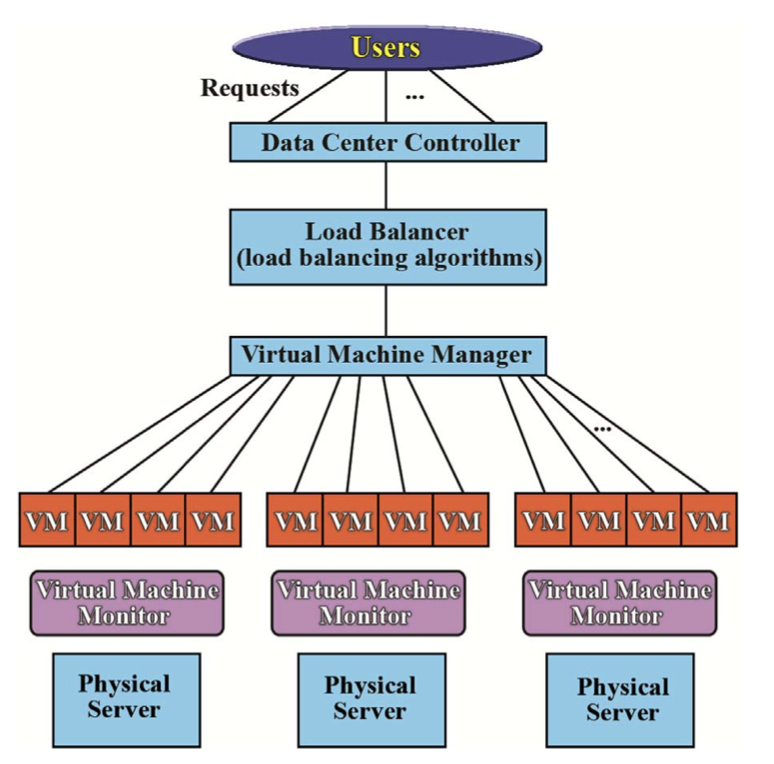
\includegraphics[width=0.5\textwidth]{images/Load_Balancing.png}
    \caption{Modell des Load Balancing}
    \label{fig:LoadBalancing}
\end{figure}

Es gibt verschiedene Arten von Load Balancing Algorithmen. Grob werden die Algorithmen aufgrund zwei verschiedener Faktoren eingeteilt: dem Zustand des Systems und der Person, die den Prozess initiert hat. 
Ersteres unterteilt sich weiter in statische und dynamische Algorithmen. Statische Algorithmen sind beispielsweise Round Robin, Min-Min oder Min Max Algorithmen. Diese setzen voraus, dass alle Systeminformationen im voraus bekannt sind. Ein Beispiel für einen fynamischen Algorithmus ist der Ant Colony Optimazation Algorithmus. Dynamische Algorithmen passen sich an die aktuelle Systemlast an und reagieren auf Änderungen in Echtzeit. 

Staische Algorithmen werden weiter in optimale und sub-optimale Algorithmen unterteilt. Optimal bedeutet, dass der Lastverteiler eine optimale Entscheidung basierend auf den vorhandenen Daten trifft. Sub-optimale Algorithmen treffen eine gute, aber nicht perfekte Entscheidung. Diese Algorithmen können heuristische oder approximative Methoden verwenden, um anpassungsfähige Entscheidungen zu treffen. Heuristische Methoden schätzen die Lösung basierend auf Erfahrungswerten, approximative Ansätze versuchen mathematisch nah an die optimale Lösung heranzukommen. 

Dynamische Algorithmen können weiter in verteilte und nicht-verteilte Klassen unterteilt werden. Bei den verteilten Algorithmen führen alle Knoten den Algorithmus aus und die Verteilung der Last ist zwischen den Knoten aufgeteilt. Zwischen den Knoten kann entweder eine kooperative oder nicht.kooperative Interaktion stattfinden. Bei der kooperativen Interaktion arbeiten die Knoten zusammen um das Ziel gemeinsam zu erreichen. Bei der nicht-kooperativen Interaktion verfolgt jeder Knoten sein eigenes lokales Ziel. Die nicht-verteilten dynamischen Algorithmen werden in zentralisierte und semi-verteilte Algorithmen unterteilt. Zentralisiert bedeutet, dass ein einzelner Knoten die Lastverteilung übernimmt. Semi-verteilt bedeutet, dass die Knoten in Gruppen organisiert sind und jeder Cluster einen zentralen Knoten hat, der für die Lastverteilung zuständig ist. 
\newline
Algorithmen, die von einer Person/einem Prozess initiert werden können entweder Sender-initiiert, Empfänger-initiiert oder symmetrisch sein.
Sender-initiiert bedeutet, dass Entscheidungen bei der Erstellung neuer Aufgaben getroffen werden. Empfänger-initiiert beudetet, dass Entscheidungen erfolgen, wenn Aufgaben abgeschlossen werden. Symmetrisch bedeutet, dass sowohl Sender als auch Empfänger Entscheidungen treffen können. \cite[S. 3]{LoadBalancing}

\subsection{Load Balancing zur Netzstabilität - Blackout}

\section{Single Point of Failure}
\subsection{Definition}
\subsection{Risiken und Auswirken}
\subsection{Angriffe auf Systeme ohne Single Point of Failure}

\bibliographystyle{plain}
\bibliography{literatur}

\end{document}
